\section{ManeFrame II (M2)}

\begin{frame}{Cluster Super Computers}
\begin{figure}
  \centering
  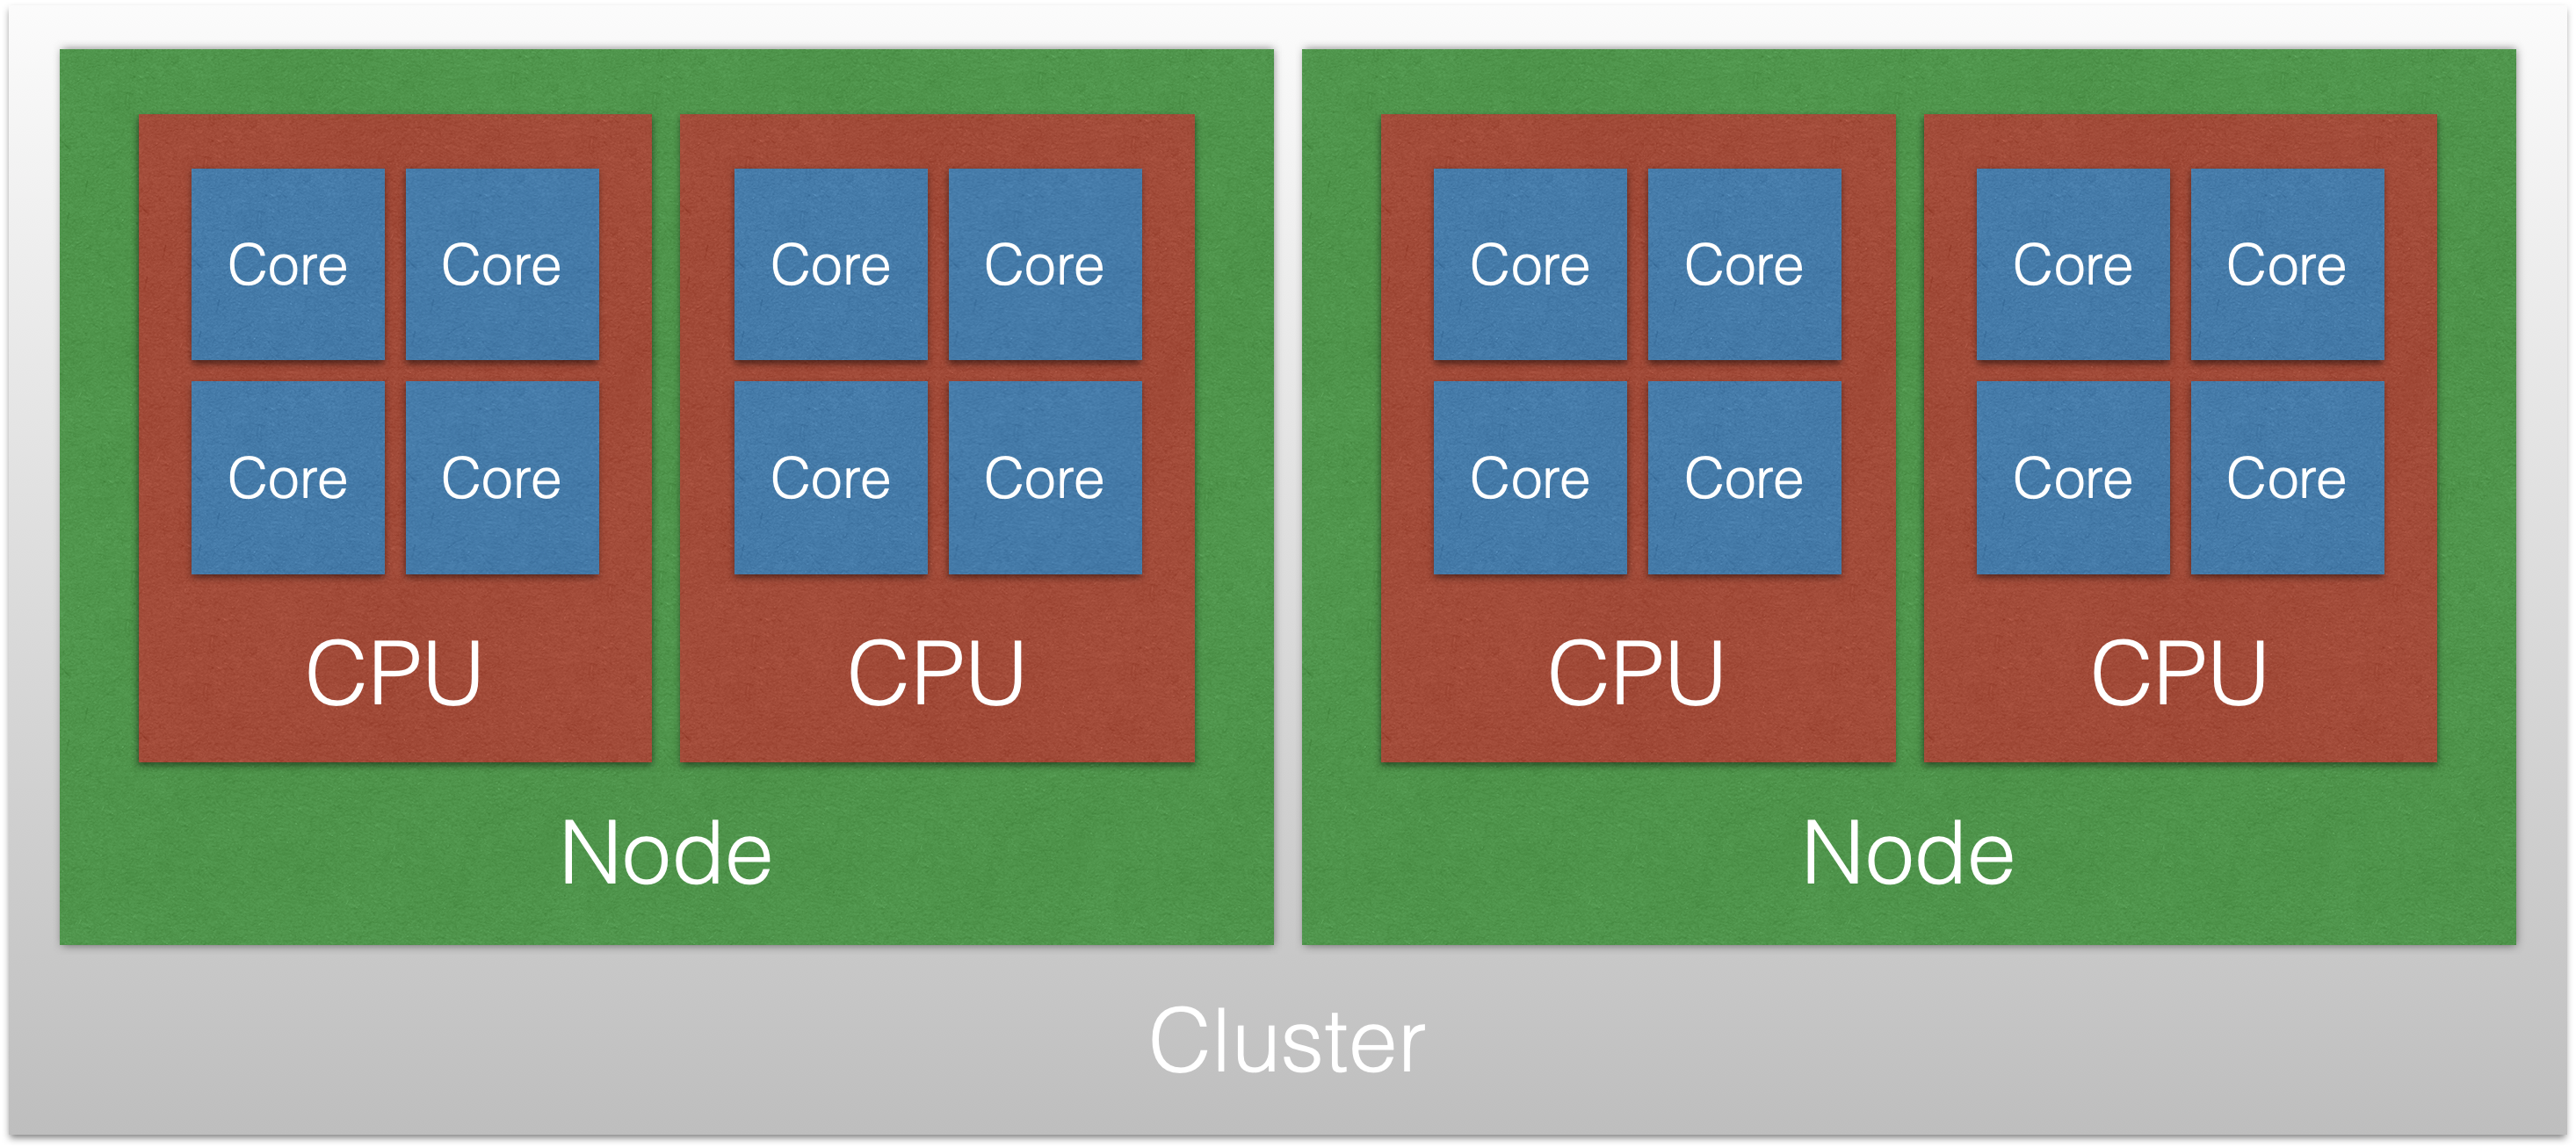
\includegraphics[width=0.75\linewidth]{figures/cluster.png}
  \caption{A cluster is a collection of individual computers networked together. Applications can be configured to run on all available compute resources.}
\end{figure}
\end{frame}

\begin{frame}{ManeFrame II (M2) Node Types}
\begin{table}
\tiny
\begin{tabular}{lllll}
\toprule
Type & Quantity & Cores & Memory [GB] & Additional Resources\\
\midrule
Standard-Memory & 176 & 36 & 256 & \\
Medium-Memory-1 & 35 & 36 & 768 & \\
Medium-Memory-2 & 4 & 24 & 768 & 3 TB SSD local scratch\\
High-Memory-1 & 5 & 36 & 1,536 & \\
High-Memory-2 & 6 & 40 & 1,536 & 3 TB SSD local scratch\\
GPGPU-1 & 36 & 36 & 256 & NVIDIA P100 GPU has 3,584 CUDA cores and 16 GB CoWoS\\
MIC-1 & 36 & 64 & 384 & 16 GB of high bandwidth (400 GB/s) stacked memory\\
VDI & 5 & 36 & 256 & NVIDIA Quadro M5000 GPU\\
v100x8 & 3 & 36 & 768 & 8 NVIDIA V100 GPUs with 5,120 CUDA cores and 32 GB CoWoS\\
Faculty Partner Nodes & 3 &  &  & Various research specific NVIDIA GPU configurations\\
\midrule
ManeFrame II & 354 & 11,276 & 120 TB & 2.8 PB storage and InfiniBand network\\
\bottomrule
\end{tabular}
\end{table}
\end{frame}

\begin{frame}{ManeFrame II (M2) Partitions (Queues)}
\begin{table}
\tiny
\begin{tabular}{llll}
\toprule
Partition & Duration & Cores & Memory [GB]\\
\midrule
development & 2 hours & various & various\\
htc & 1 day & 1 & 6\\
standard-mem-s & 1 day & 36 & 256\\
standard-mem-m & 1 week & 36 & 256\\
standard-mem-l & 1 month & 36 & 256\\
medium-mem-1-s & 1 day & 36 & 768\\
medium-mem-1-m & 1 week & 36 & 768\\
medium-mem-1-l & 1 month & 36 & 768\\
medium-mem-2 & 2 weeks & 24 & 768\\
high-mem-1 & 2 weeks & 36 & 1538\\
high-mem-2 & 2 weeks & 40 & 1538\\
mic & 1 week & 64 & 384\\
gpgpu-1 & 1 week & 36 & 256\\
v100x8 & 1 week & 1 & 20\\
fp-gpgpu-2 & various & 24 & 128\\
fp-gpgpu-3 & various & 40 & 384\\
\bottomrule
\end{tabular}
\end{table}
\end{frame}

\begin{frame}{ManeFrame II File Systems}
\begin{description}
\item[\$HOME]
\begin{itemize}
  \item Default file system when logging into M2, e.g. \mintinline{sh}{/users/$USER}.
  \item Space should be used to write, edit, compile programs, and job submission scripts, etc.
  \item Restricted by quotas (200 GB) and backed-up.
\end{itemize}
\item[\$WORK]
\begin{itemize}
  \item Long term storage at \mintinline{sh}{/work/users/$USER}.
  \item Restricted by quotas (8 TB) and not backed-up.
\end{itemize}
\item[\$SCRATCH]
\begin{itemize}
 \item Scratch space at \mintinline{sh}{/scratch/users/$USER}.
 \item Treat \$SCRATCH as a volatile file system that is not backed-up.
\end{itemize}
\end{description}
\end{frame}

